\subsection{Planck CMB lensing maps}

Using the most recent reconstructed lensing convergence maps and analysis masks provided in the Planck 2018 release\footnote{\url{https://wiki.cosmos.esa.int/planck-legacy-archive}} \citep{PlanckVIII}, we focus mainly on the baseline estimates obtained from the SMICA DX12 CMB maps with a minimum-variance (MV) estimate determined from both the temperature and polarization maps. To gauge the impact of the thermal Sunyaev-Zeldovich (tSZ) effect, which has been shown to bias the lensing reconstruction and contaminate cross-correlations with other tracers of large-scale structure (see e.g. \citealt{Osborne++14, vanEngelen++14, Madhavacheril++18, Schaan++19}), we also repeat the analysis using the lensing estimate obtained from a temperature-only SMICA map where tSZ has been deprojected using multifrequency component separation. Throughout the remainder of this paper, these two lensing maps will be referred to as \texttt{BASE} and \texttt{DEPROJ}, respectively. 

The spherical harmonic coefficients of the reconstructed lensing convergence maps are provided in HEALPix\footnote{\url{http://healpix.sf.net}} \citep{Gorski++05} format with maximum order $\ell_{\text{max}}=4096$, and the associated analysis masks are given as HEALPix maps with resolution $N_{\text{SIDE}} = 2048$. The approximate lensing noise power spectrum for the fiducial cosmology used in \cite{PlanckVIII} is also provided up to $\ell_{\rm max} = 4096$.

\subsection{Photometric DESI LRGs}

The Dark Energy Spectroscopic Instrument (DESI; \citealt{DESI16}) is an upcoming Stage IV\footnote{As defined in the Dark Energy Task Force report \citep{DarkEnergyTaskForce}.} dark energy experiment, installed on the Mayall 4m telescope at Kitt Peak. DESI aims to produce the largest ever three-dimensional map of the universe, with a massively multiplexed spectrograph that uses robotic fiber positioners to measure as many as 5000 spectra in parallel. Among the four main classes targeted by DESI are luminous red galaxies (LRGs) out to $z \approx 1$. LRGs, as their name suggests, are luminous and intrinsically red due to their high stellar mass and lack of recent star formation activity. LRGs are excellent tracers of large-scale structure; as early-type galaxies with generally old populations of stars, they are expected to reside in massive halos and therefore cluster strongly. Furthermore, their inherent brightness and the strong 4000\AA \ feature in their spectral energy distributions enable the efficient selection of a homogeneous sample using photometry.

\subsubsection{DECaLS imaging data}

%https://arxiv.org/pdf/1906.00970.pdf

The DECam Legacy Survey (DECaLS) is a deep, wide-field survey providing the optical imaging used to conduct targeting for approximately two-thirds of the DESI footprint, covering the region bounded by $\delta \lesssim 32^{\circ}$. Through the DECam instrument \citep{Flaugher15} on the Blanco 4m telescope, DECaLS observes in three optical and near-IR bands ($g$, $r$, $z$), with four additional mid-IR bands ($W1$, $W2$, $W3$, $W4$) provided by the Wide-field Infrared Survey Explorer (WISE; \citealt{Wright10}). DECam images are processed and calibrated though the National Optical Astronomy
Observatory (NOAO) Community Pipeline, then fed into \textit{The Tractor}\footnote{\url{https://github.com/dstndstn/tractor}} \citep{Lang16a}, which uses forward-modeling to perform source extraction and produce probabilistic inference of source properties.


%Raw DECam images are processed through the NOAO Community Pipelines, with astrometric calibration and photometric characterization based on Pan-STARRS-1 measurements. The calibrated images are then run through \textit{The Tractor}\footnote{\url{https://github.com/dstndstn/tractor}} \citep{Lang16a}, which produces an inference-based catalog by optimizing the likelihood for source properties, given the data and a noise model.

Our analysis is based on Data Release 8 (DR8), the latest data release of the Legacy Survey \citep{Dey18}, which contains DECaLS observations from August 2014 through March 2019 (NOAO survey program 0404). DR8 also includes some non-DECaLS observations from the DECam instrument, mainly from the Dark Energy Survey (DES; \citealt{DES05}). In total, the DECaLS +DES portion of DR8 covers approximately 14,996 square degrees in the $g$-band, 15,015 square degrees in the $r$-band, 15,130 square degrees in the $z$-band, and 14,781 square degrees in all three optical bands jointly.\footnote{Estimated from using randoms distributed uniformly across the footprint to sum up the areas with at least one exposure in each band.} 

\subsubsection{Galaxy selection}\label{sec:data:ts}

DESI LRGs are selected from DECaLS by applying a complex series of color cuts on extinction-corrected magnitudes in $g$, $r$, $z$, and $W1$ bands:

\begin{equation}
\begin{split}
z_{\rm fiber} &< 21.5 \\ %
r - z &> 0.7 \\ %
(z - W1) > 0.8 &\ (r - z) - 0.6 \\ %
((g - W1 > 2.6) \text{ AND } (g - r > &1.4)) \text{ OR } (r - W1 > 1.8) \\ % 
(r - z > (z - 16.83) \ 0.45) \text{ AND } &(r - z > (z - 13.80) \ 0.19) \\%
\end{split}
\end{equation} \\ 
We note that the faint magnitude limit uses fiber flux, which is defined as the flux within a 1.5 arcsec diameter circular aperture centered on the model convolved with a 1.0 arcsec FWHM Gaussian. Color-color plots of the resulting sample are displayed in Figure~\ref{fig:colorcolor}.
%
%We can further split the LRGs into two subsamples with different mean redshifts by applying an additional photometric cut. Motivated by eBOSS studies, \textcolor{red}{Kitanidis et al. 2019} divided the DESI LRG catalog along $r-W1=2.6$ and calculated the clustering $dN/dz$ for each, showing that the result is two subsamples of approximately equal size, with one at $\bar{z} \approx 0.5$ and the other at $\bar{z} \approx 0.8$. This binning is also helpful for minimizing the effect of bias evolution in the clustering $dN/dz$ estimation \citep{Menard13, Schmidt13, Rahman15, Gatti18}.

\begin{figure}
\centering
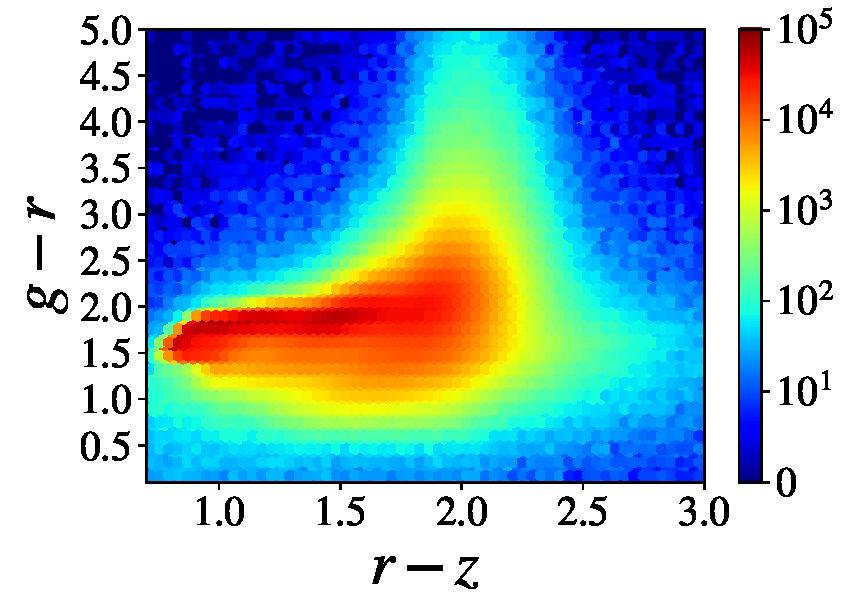
\includegraphics[width=0.7\columnwidth, trim={0.35cm 0 0 0},clip]{figures/LRG_colorcolor_grz.pdf}
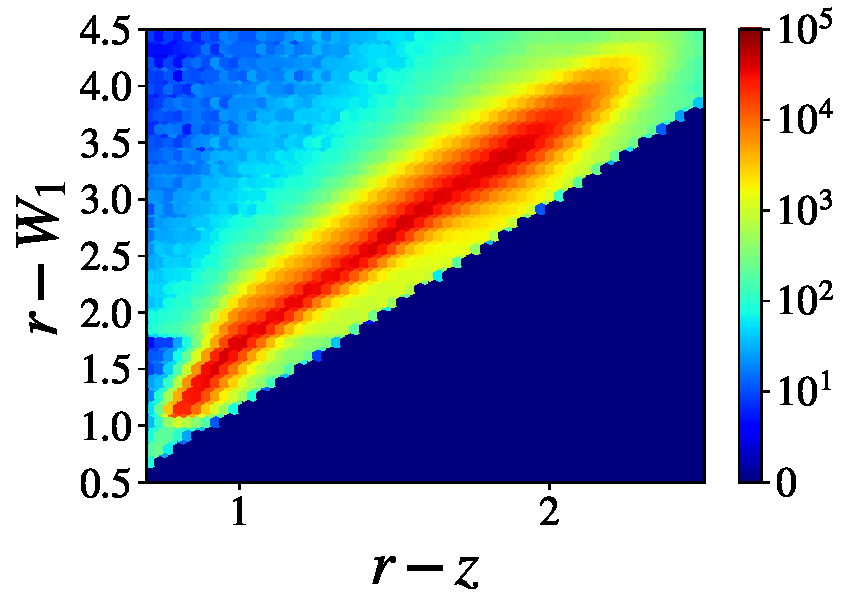
\includegraphics[width=0.7\columnwidth, trim={0.35cm 0 0 0},clip]{figures/LRG_colorcolor_rzW1.pdf}
\caption{Color-color plots of the LRG target selection in DECaLS DR8, with the color bar representing the total number of targets.}
\label{fig:colorcolor}
\end{figure}


\subsubsection{Masks}
\label{sec:data:masks}

Instrument effects and transients create artifacts in the images which may impact the detection or fitting of sources. Additionally, bright foregrounds, including point sources such as stars and extended sources such as large galaxies, globular clusters, and planetary nebulae, can contaminate the pixels around them with false targets, thereby affecting the apparent angular distribution of the target sample. DR8 provides bitmasks which leverage the NOAO Community Pipeline's data quality map, as well as several external catalogs, to reject bad pixels and mask around foregrounds. The bits we use in our analysis are summarized in Table~\ref{tab:masks} and briefly described below:


The \texttt{ALLMASK\_X} bits are set for pixels that touch a bad pixel (as flagged by the NOAO Community Pipeline) in all of the overlapping $X$-band images. The \texttt{WISEM1} and \texttt{WISEM2} bits are set for pixels that touch a pixel in a mask around bright stars from the WISE catalog, with the two masks using the $W1$ and $W2$ bands, respectively. The \texttt{MEDIUM} bit is set for pixels that touch a pixel containing a medium-bright ($\texttt{phot\_g\_mean\_mag} < 16$) star from the Gaia DR2 catalog \citep{GaiaDR2} or a bright ($VT < 13$) star from the Tycho-2 catalog \citep{Hog00}. The \texttt{GALAXY} bit is set for pixels that touch a pixel containing a large galaxy, where the source catalog used for this mask is taken from John Moustakas' Legacy Survey Large Galaxy Atlas\footnote{\url{https://github.com/moustakas/LSLGA}} work with Dustin Lang. Finally, clusters and nebulae from OpenNGC\footnote{\url{https://github.com/mattiaverga/OpenNGC}} are masked around using a circular mask whose diameter is equal to the major axis of the object being masked, and the \texttt{CLUSTER} bit is set for pixels touching this mask.

As demonstrated in Table~\ref{tab:masks}, masking near foreground stars causes the largest cut in observed objects. To determine whether any additional stellar masking is warranted, we measure the density of targets as a function of proximity to stars after the above bitmasks have been applied. Using the Tycho-2 and WISE catalogs, we first bin the stars by their magnitudes (using the $VT$ and $W1$ bands, respectively), and then determine the density of LRGs in annular bins around these stacks of stars. We find that there are still residual effects near Tycho-2 stars, particularly for the brightest bins, that are not entirely captured by the bitmasks. We find even more significant effects around WISE stars, with the LRG density peaking beyond the radius of the bitmasks. We fit a magnitude-dependent masking radius for each star catalog to apply as additional geometric masks: 
%
\begin{align}\label{eq:mr-veto}
R = 
\begin{cases}
    10^{\ 3.41 \ - \ 0.16 \ \times \ VT} \ \text{arcsec}, \hspace{0.5cm} \text{Tycho-2} \\
    10^{\ 2.87 \ - \ 0.13 \ \times \ W1} \ \text{arcsec}, 
    \hspace{0.5cm} \text{WISE}
\end{cases}
\end{align}
%
The addition of the geometric masks results in a slight increase in the total masked area.
%
\begin{table}
    {\centering
\noindent\begin{tabular}{p{1.0cm}p{1.5cm}p{1.3cm}p{1.4cm}p{0.6cm}}
\toprule
\multicolumn{2}{c}{Mask} & Number & Area (deg$^2$) & $f_{\rm survey}$ \\
\hline
\multicolumn{2}{c}{\textbf{no masks}} & 9003243 & 14610.72 & 1.000 \\
\hline
\multirow{8}{*}{bits}    & \texttt{ALLMASK\_G}  & 9002762 & 14610.72 & 1.000 \\
                          & \texttt{ALLMASK\_R}  & 9002742 & 14610.72 & 1.000 \\
                          & \texttt{ALLMASK\_Z}  & 9002458 & 14610.72 & 1.000 \\
                          & \texttt{WISEM1}  & 8578461 & 14230.96 & 0.974 \\
                          & \texttt{WISEM2}  & 8679070 & 14406.05 & 0.986 \\
                          & \texttt{MEDIUM}  & 8566358 & 13945.27 & 0.954 \\
                          & \texttt{GALAXY}  & 8996317 & 14599.17 & 0.999 \\
                          & \texttt{CLUSTER} & 9003232 & 14609.73 & 1.000 \\
\cmidrule{2-5}
                          & all bits     & 8559863 & 13933.29 & 0.954 \\
\hline
\multirow{2}{*}{geometric} & Tycho-2  & 8675511 & 14181.29 & 0.971 \\
                           & WISE    & 8488111 & 14094.18 & 0.965 \\
\cmidrule{2-5}
                           & all geometric    & 8399015 & 13859.42 & 0.949 \\
\hline
\multicolumn{2}{c}{\textbf{all masks}} & 8390823 & 13851.50 & 0.948 \\
\bottomrule
\end{tabular}}
    \caption{Summary of foreground masks.}
    \label{tab:masks}
\end{table}

\subsubsection{Tests of potential systematics}

Astrophysical foregrounds, poor observing conditions, and systematic errors in instrument calibration or data reduction can introduce non-cosmological density variations in the galaxy sample, which may in turn bias cosmological analyses (see e.g.\ \citealt{Myers06}, \citealt{Crocce11}, \citealt{Ross11}, \citealt{Suchyta++16}, \citealt{Crocce++16}, \citealt{Leistedt++16}, \citealt{ElvinPoole18}, \citealt{Ross20}, \citealt{Weaverdyck20} for studies of imaging systematics in the context of other surveys). A full analysis of the effect of imaging systematics  on the clustering of DESI main targets using data from DECaLS DR7 is presented in \citealt{Kitanidis++19}. Here, we briefly perform tests of the LRG density dependence on these potential systematics using DR8 data and target selection.  

We use the \texttt{HEALPix} scheme with $N_{\text{SIDE}} = 256$ to divide the footprint into pixels of equal area, over which we average each systematic. This resolution is chosen to ensure most pixels contain $>10$ galaxies, for better statistics. These pixelised maps are shown in Figure~\ref{fig:systematic_maps}. The survey properties we look at are stellar density, galactic extinction, airmass, seeing, sky background, and exposure time. For full descriptions of these survey properties, how they are calculated, and why they are included in the analysis, see Section 6 of \citealt{Kitanidis++19}. 

For each map, we bin the pixels by the value of the survey property, and then determine the average density per bin. The resulting plots of LRG density contrast $\delta = n/\bar{n} - 1$ as a function of survey properties are shown in Figure~\ref{fig:systematic_trends}, with the cumulative sky fractions shown in the upper panels and the dotted lines corresponding to 1\% fluctuations. We show that LRG density variation due to systematic sources of error are controlled to within 5\% and, more often than not, 1\%. As such, we conclude that imaging systematics should not significantly affect our cross-correlation measurements.

%\EK{Based on feedback from other paper, maybe we want to split this by NGC vs SGC. Also based on feedback from previous paper, maybe write a note about our choice of resolution.}

\begin{figure*}
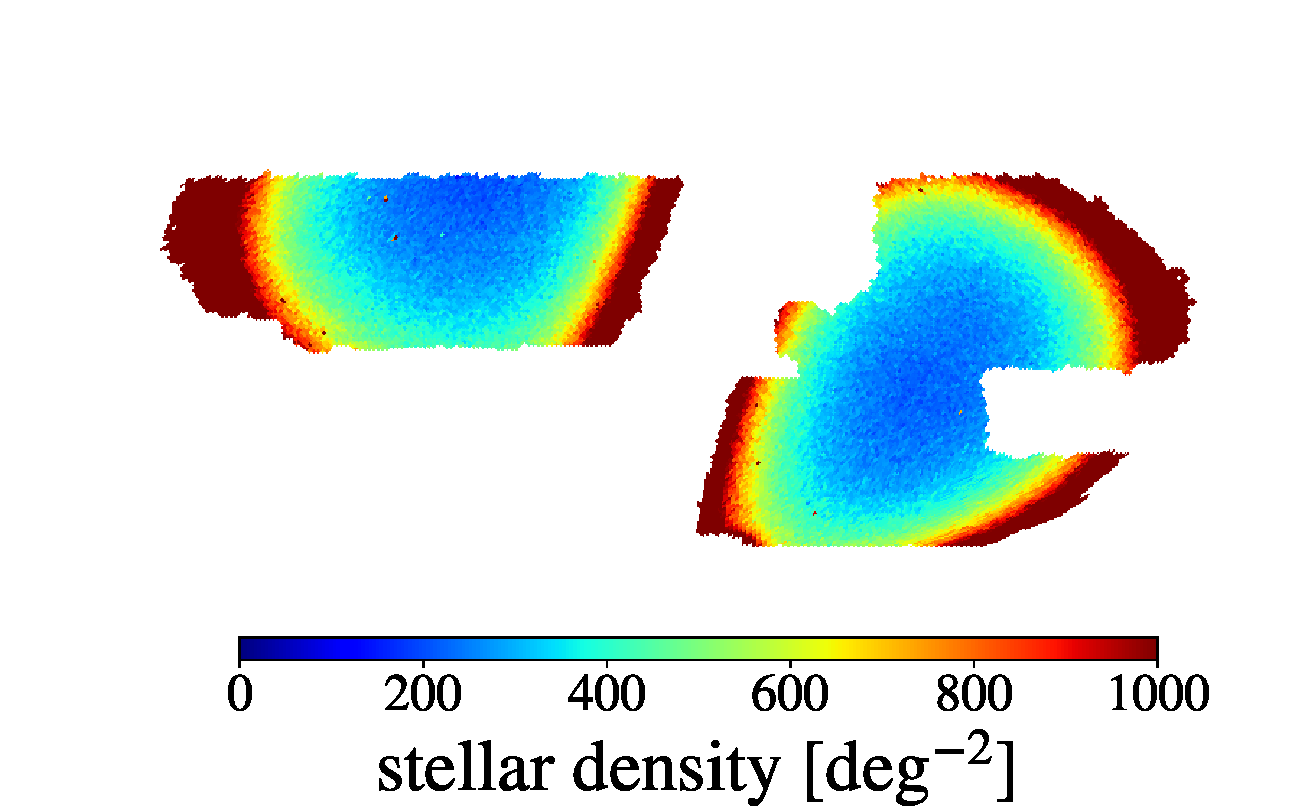
\includegraphics[width=0.24\linewidth, trim={1.5cm 0 1.2cm 1.5cm},clip]{figures/systematic_maps/stellar.pdf}
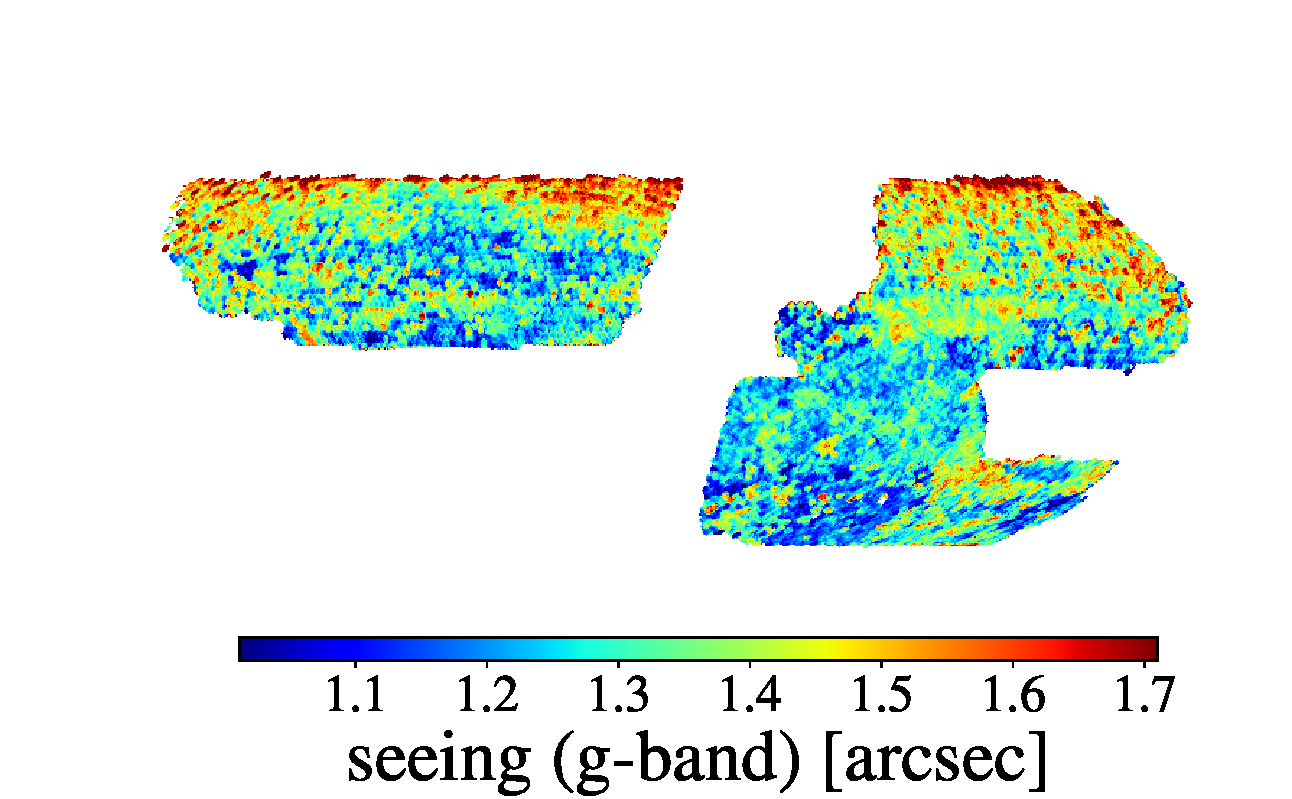
\includegraphics[width=0.24\linewidth, trim={1.5cm 0 1.2cm 1.5cm},clip]{figures/systematic_maps/seeing_g.pdf}
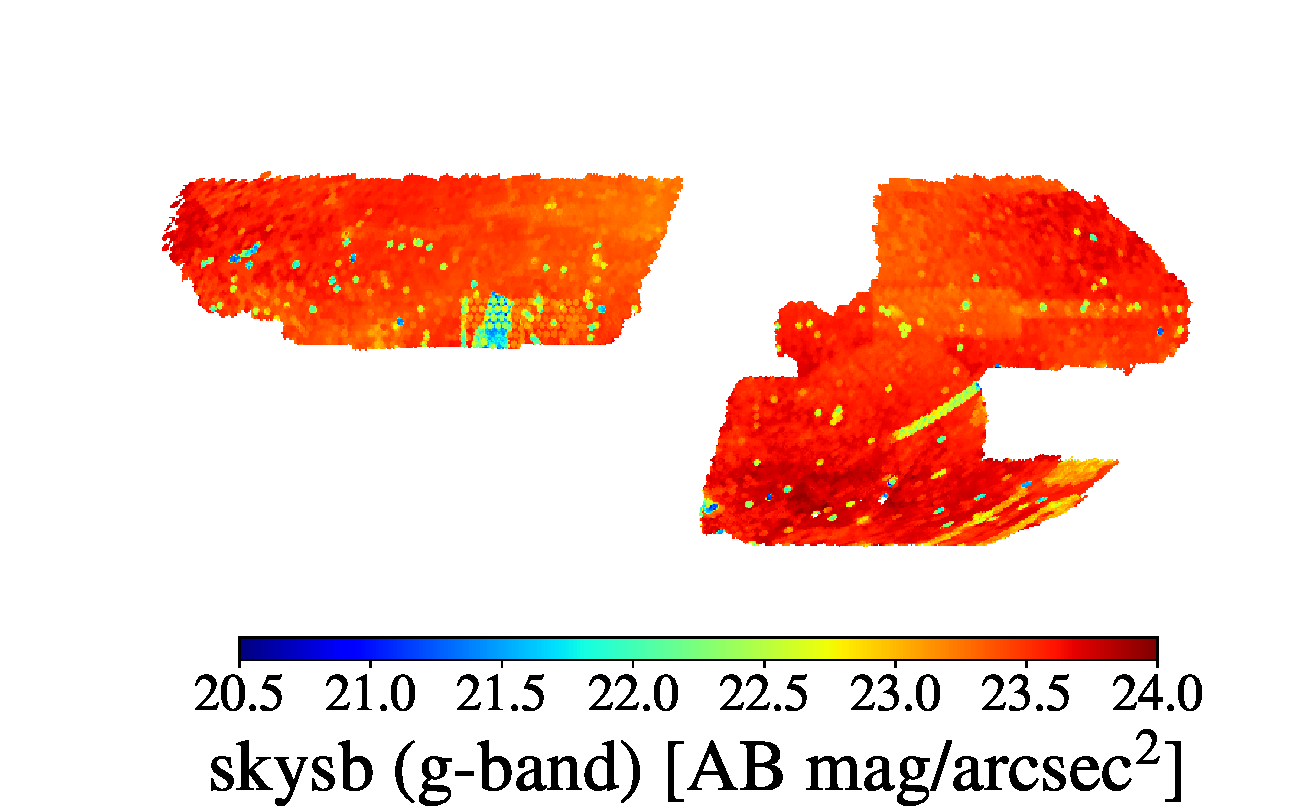
\includegraphics[width=0.24\linewidth, trim={1.5cm 0 1.2cm 1.5cm},clip]{figures/systematic_maps/skymag_g.pdf}
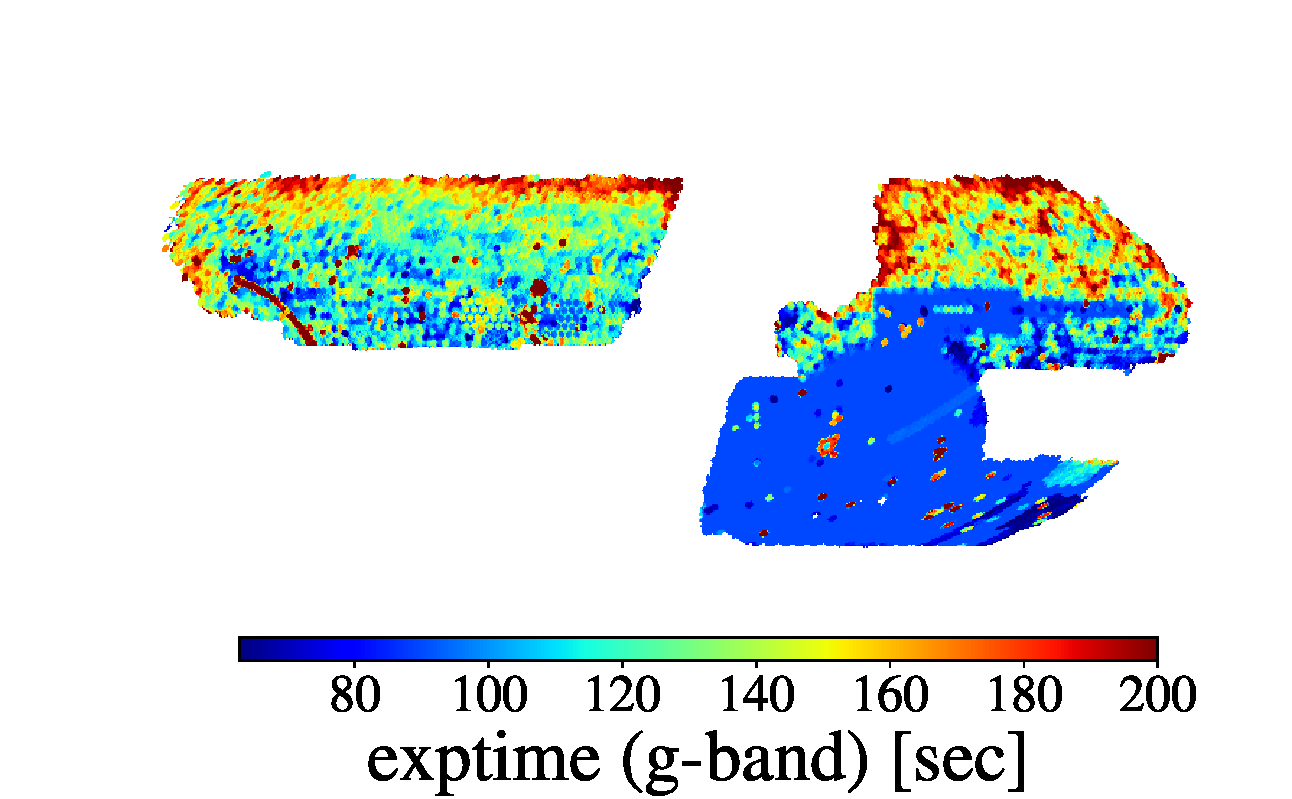
\includegraphics[width=0.24\linewidth, trim={1.5cm 0 1.2cm 1.5cm},clip]{figures/systematic_maps/exptime_g.pdf}
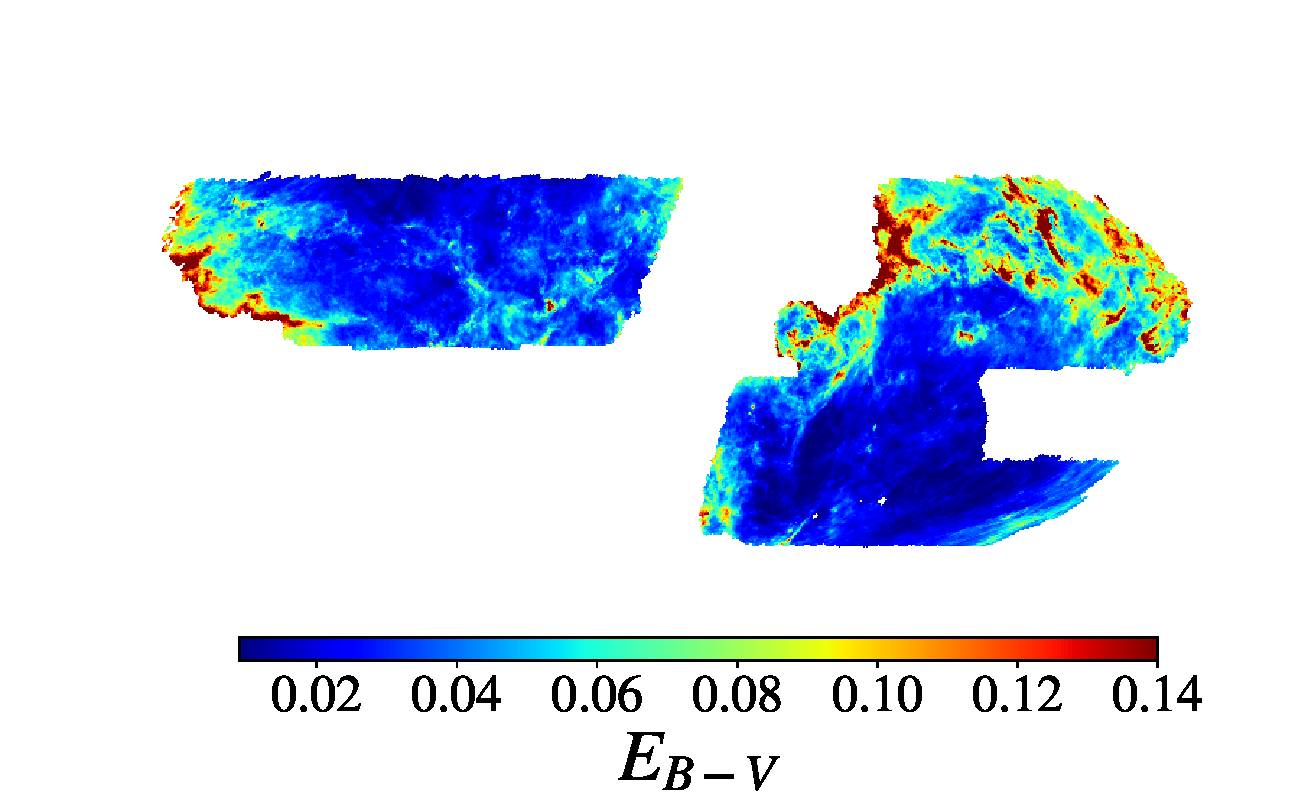
\includegraphics[width=0.24\linewidth, trim={1.5cm 0 1.2cm 1.5cm},clip]{figures/systematic_maps/ebv.pdf}
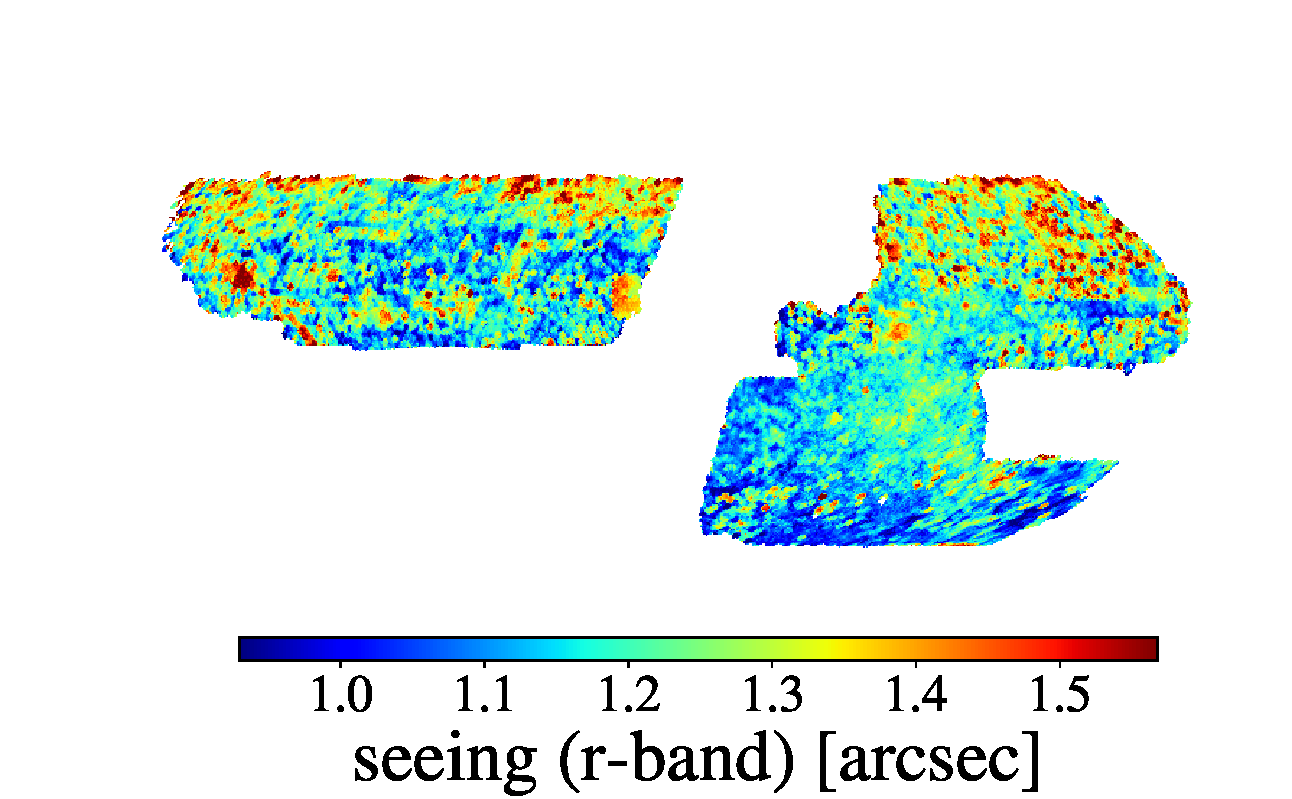
\includegraphics[width=0.24\linewidth, trim={1.5cm 0 1.2cm 1.5cm},clip]{figures/systematic_maps/seeing_r.pdf}
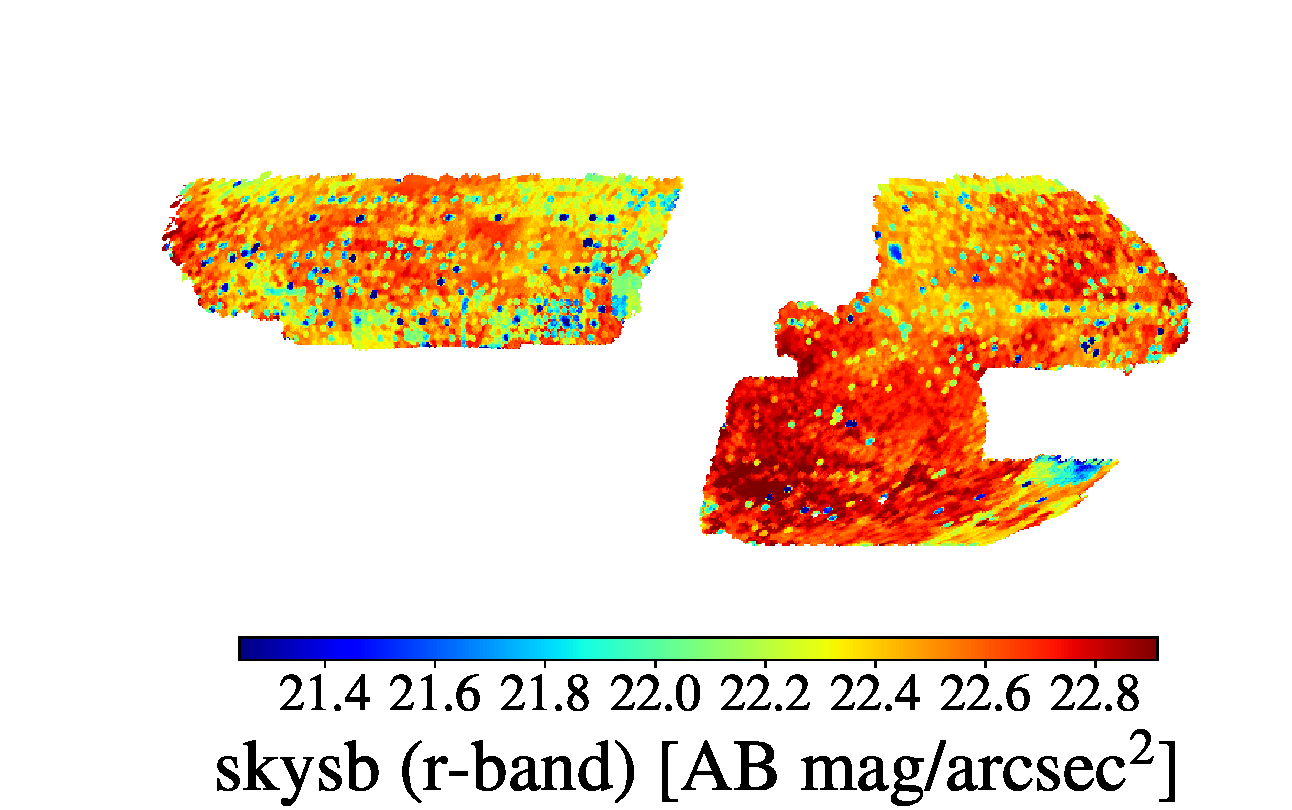
\includegraphics[width=0.24\linewidth, trim={1.5cm 0 1.2cm 1.5cm},clip]{figures/systematic_maps/skymag_r.pdf}
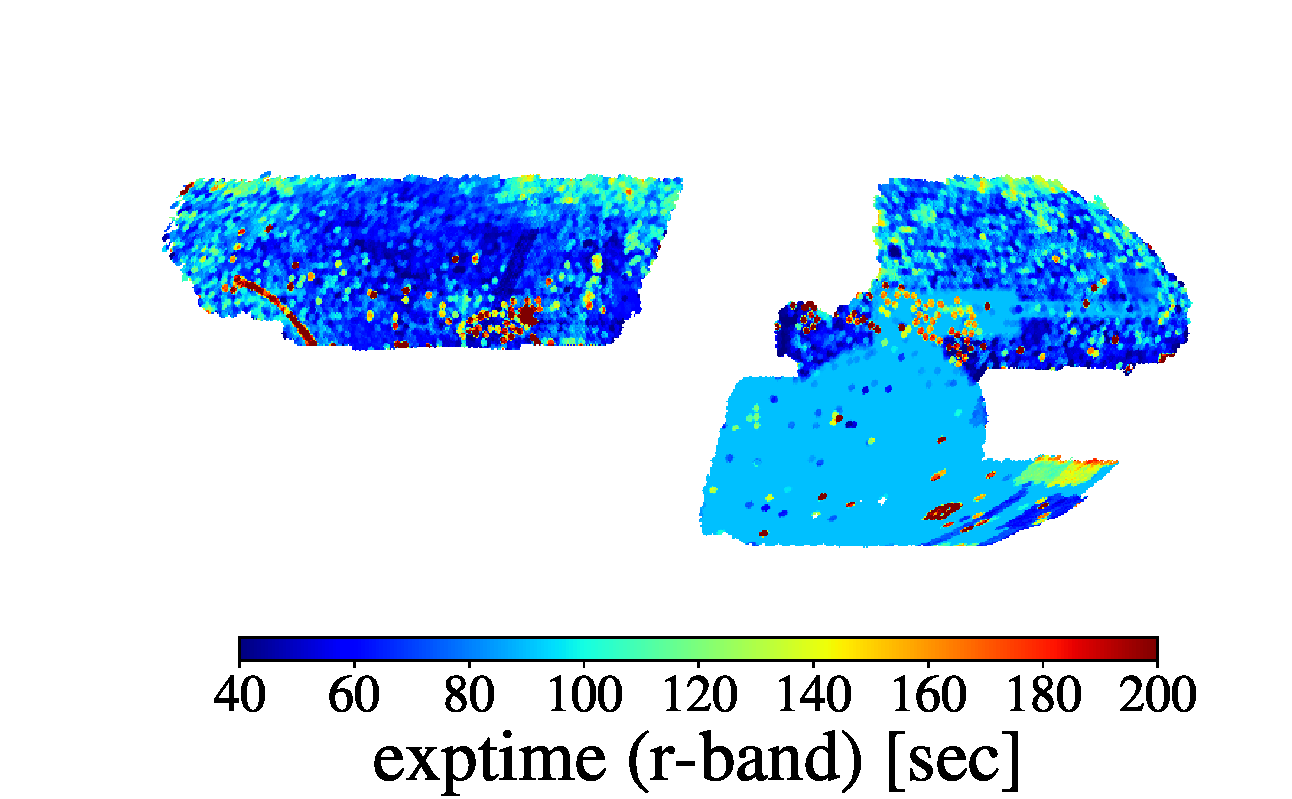
\includegraphics[width=0.24\linewidth, trim={1.5cm 0 1.2cm 1.5cm},clip]{figures/systematic_maps/exptime_r.pdf}
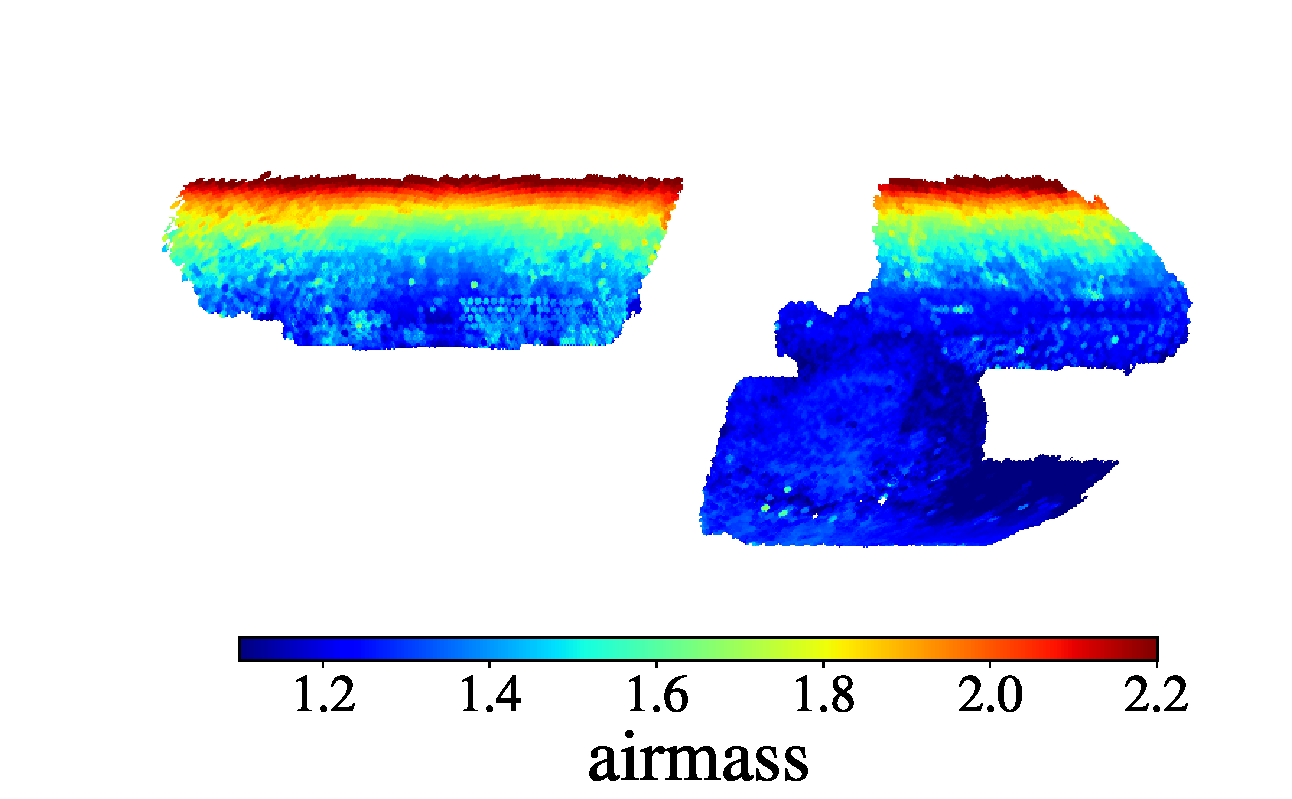
\includegraphics[width=0.24\linewidth, trim={1.5cm 0 1.2cm 1.5cm},clip]{figures/systematic_maps/airmass.pdf}
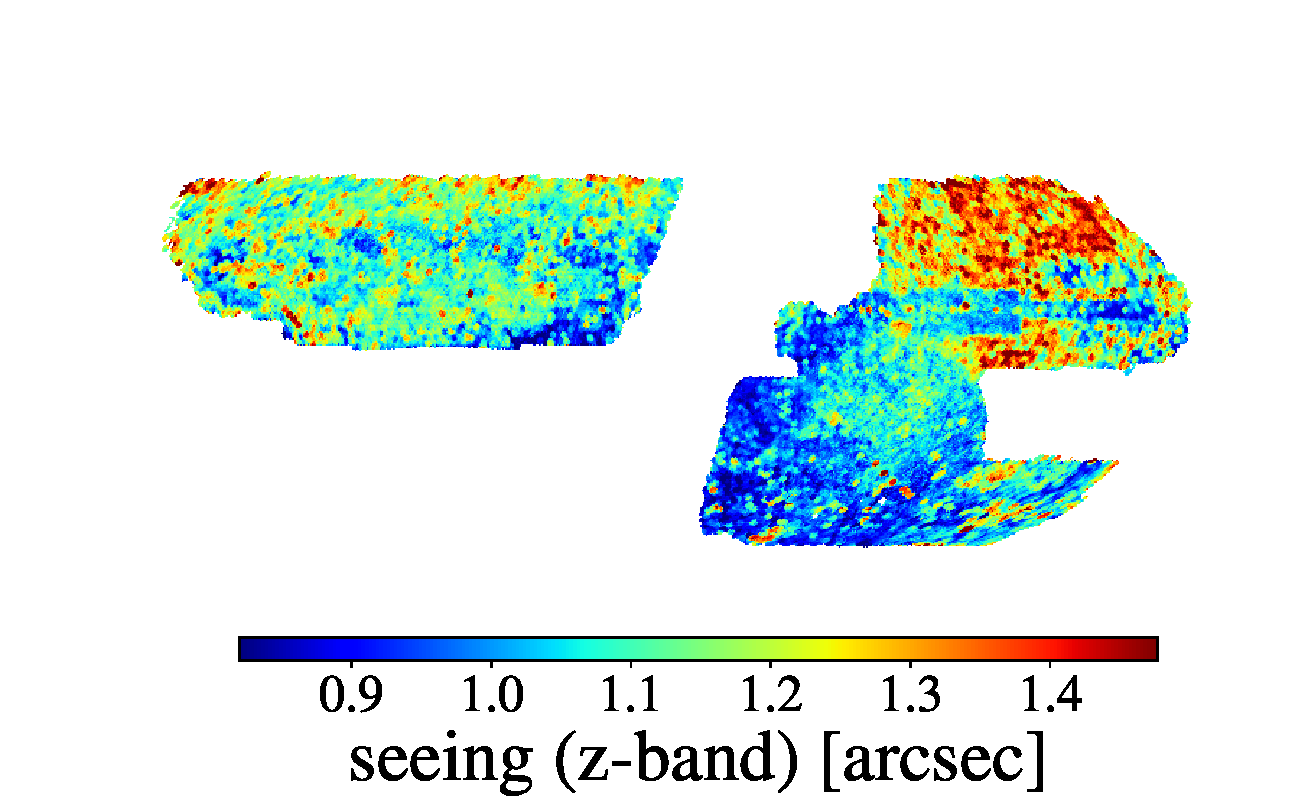
\includegraphics[width=0.24\linewidth, trim={1.5cm 0 1.2cm 1.5cm},clip]{figures/systematic_maps/seeing_z.pdf}
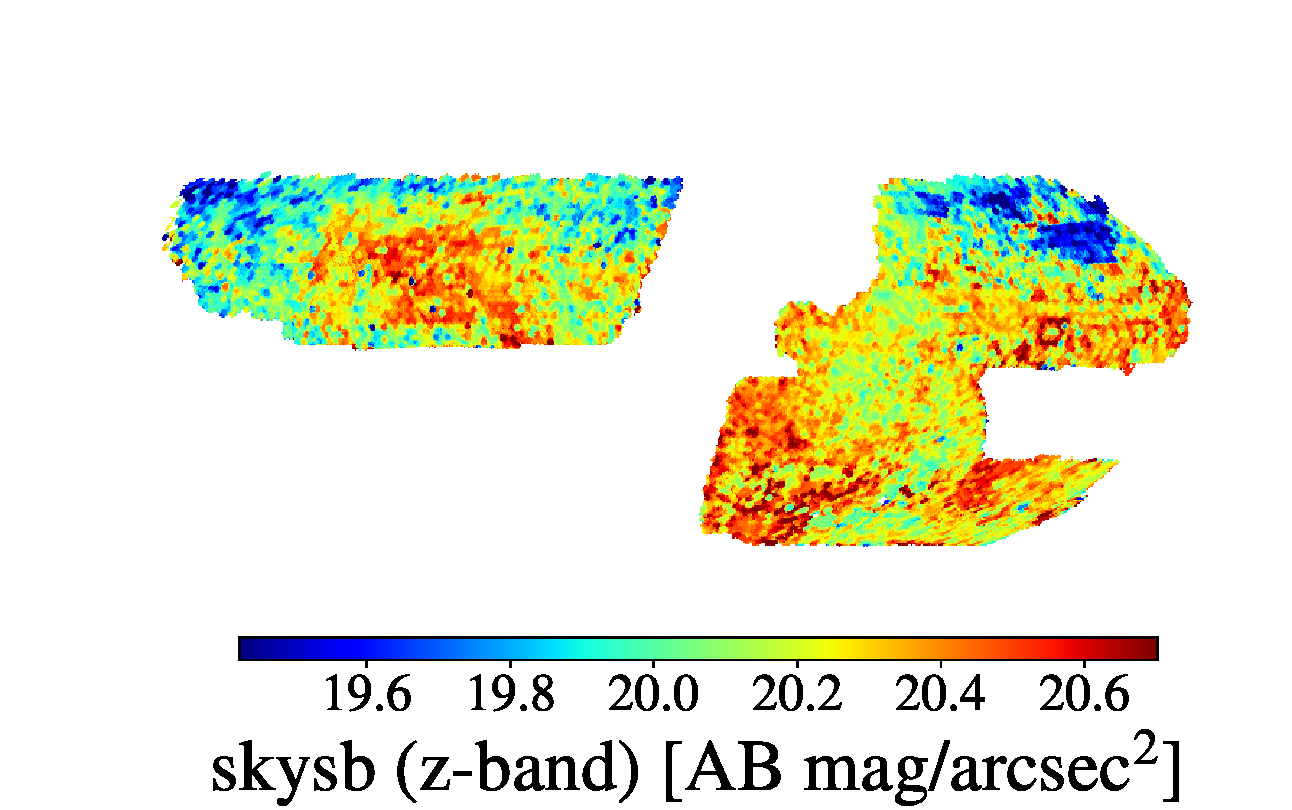
\includegraphics[width=0.24\linewidth, trim={1.5cm 0 1.2cm 1.5cm},clip]{figures/systematic_maps/skymag_z.pdf}
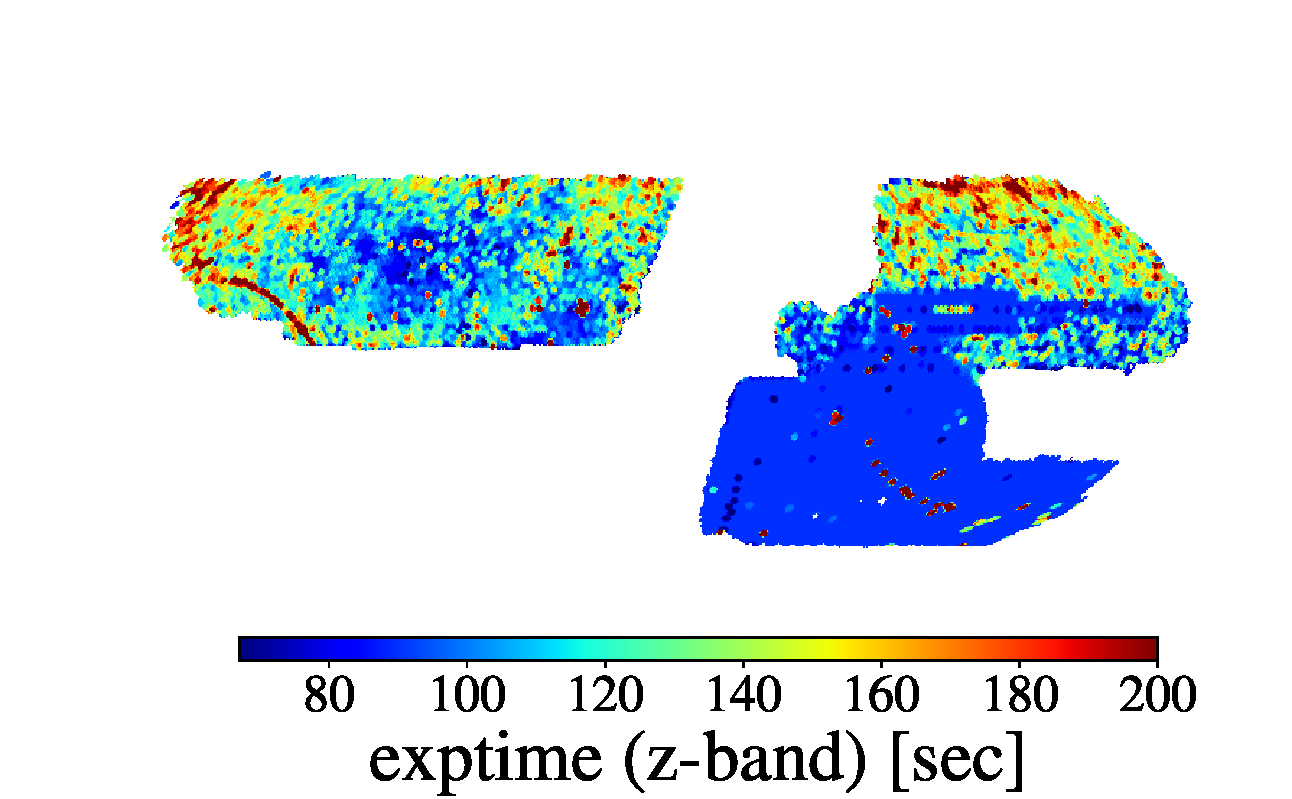
\includegraphics[width=0.24\linewidth, trim={1.5cm 0 1.2cm 1.5cm},clip]{figures/systematic_maps/exptime_z.pdf}
\caption{Maps of spatially-varying potential systematics in equatorial coordinates with Mollweide projection and the astronomy convention (east towards left).}
\label{fig:systematic_maps}
\end{figure*}

\begin{figure*}
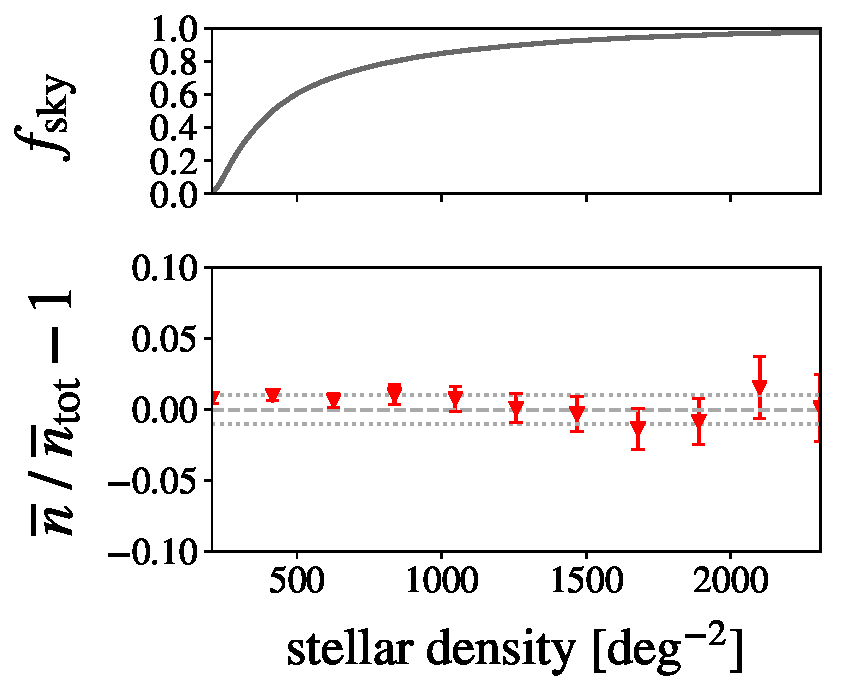
\includegraphics[width=0.24\linewidth]{figures/systematic_trends/stellar.pdf}
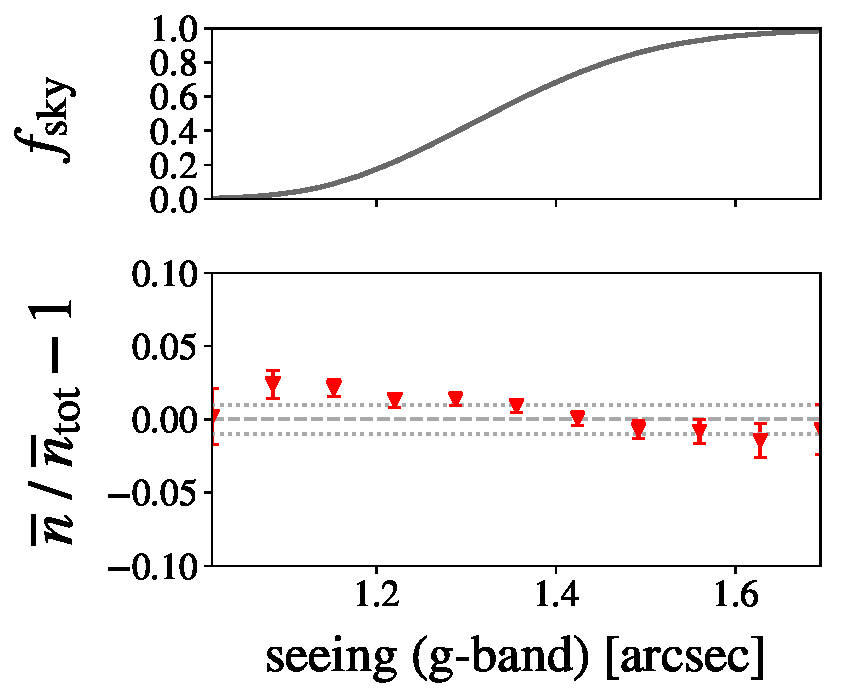
\includegraphics[width=0.24\linewidth]{figures/systematic_trends/seeing_g.pdf}
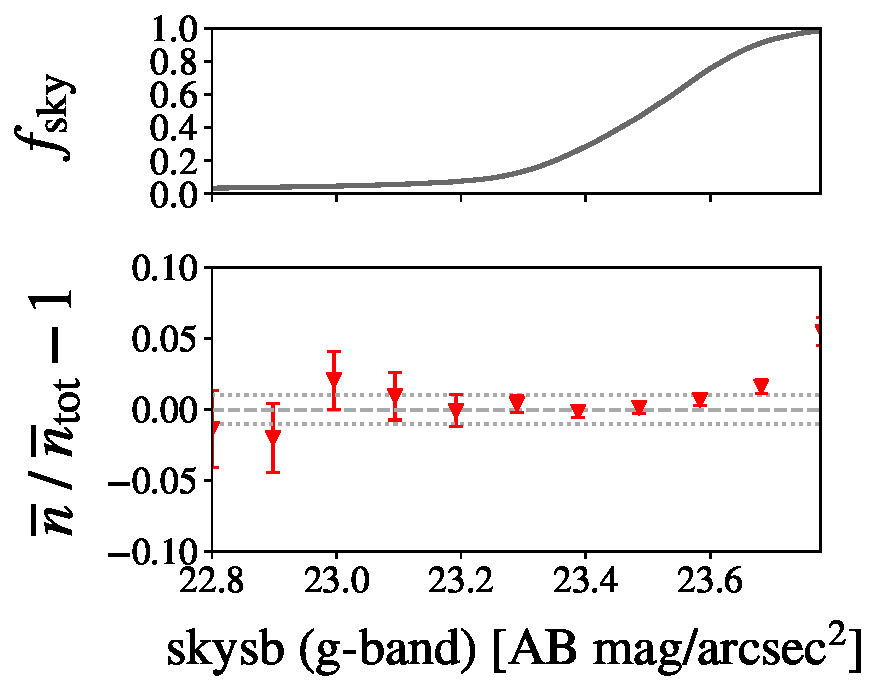
\includegraphics[width=0.24\linewidth]{figures/systematic_trends/skymag_g.pdf}
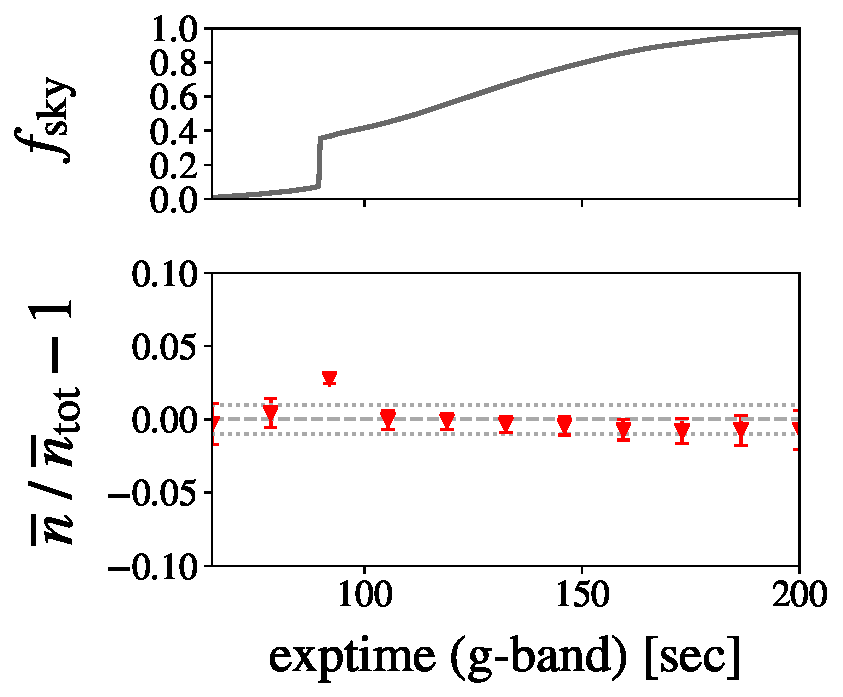
\includegraphics[width=0.24\linewidth]{figures/systematic_trends/exptime_g.pdf}
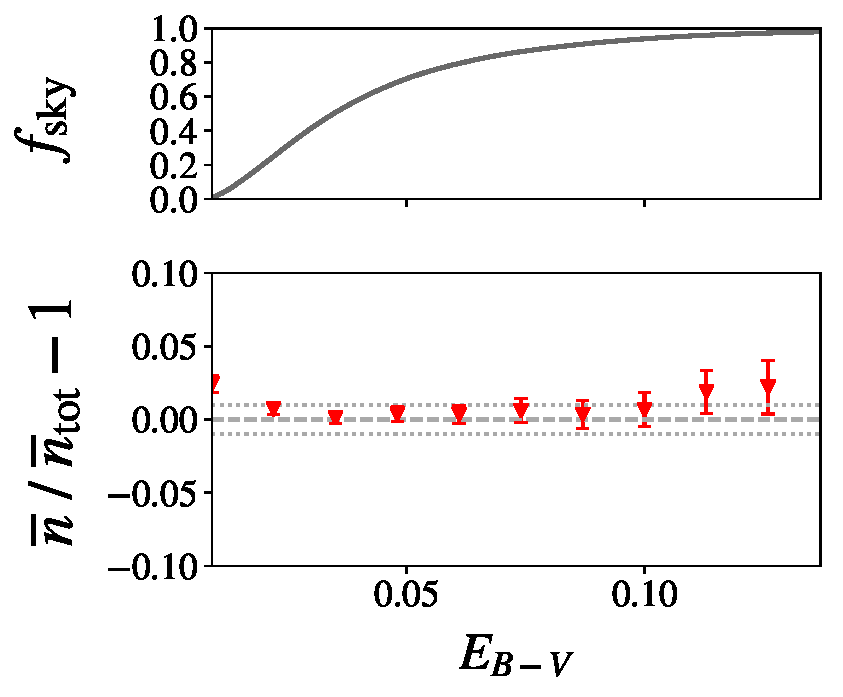
\includegraphics[width=0.24\linewidth]{figures/systematic_trends/ebv.pdf}
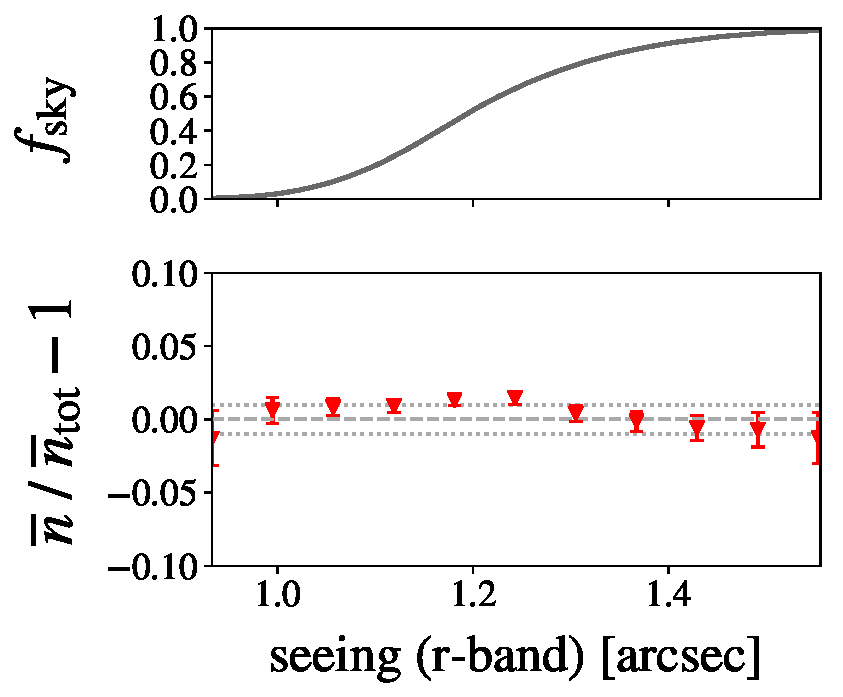
\includegraphics[width=0.24\linewidth]{figures/systematic_trends/seeing_r.pdf}
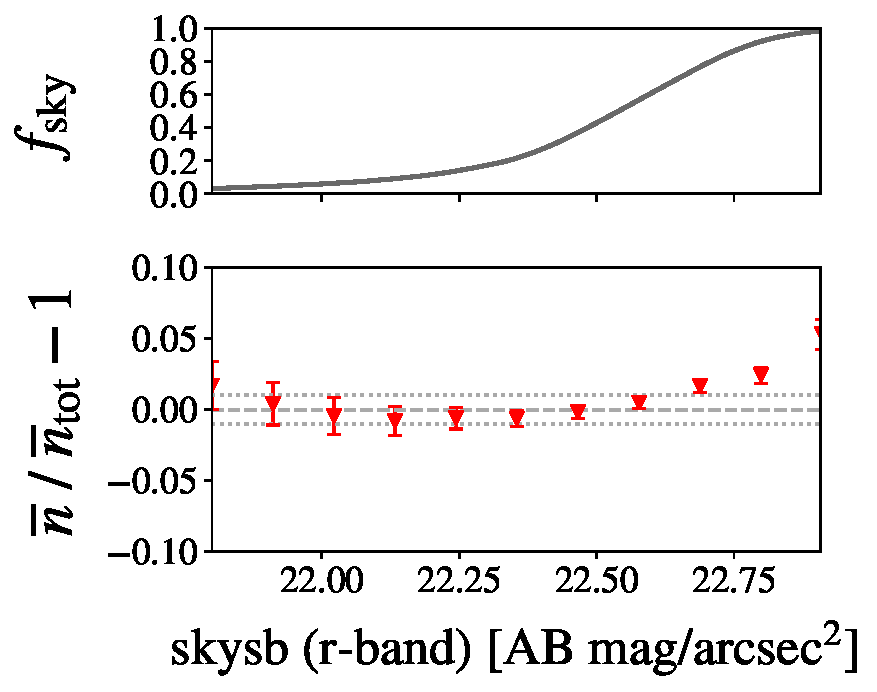
\includegraphics[width=0.24\linewidth]{figures/systematic_trends/skymag_r.pdf}
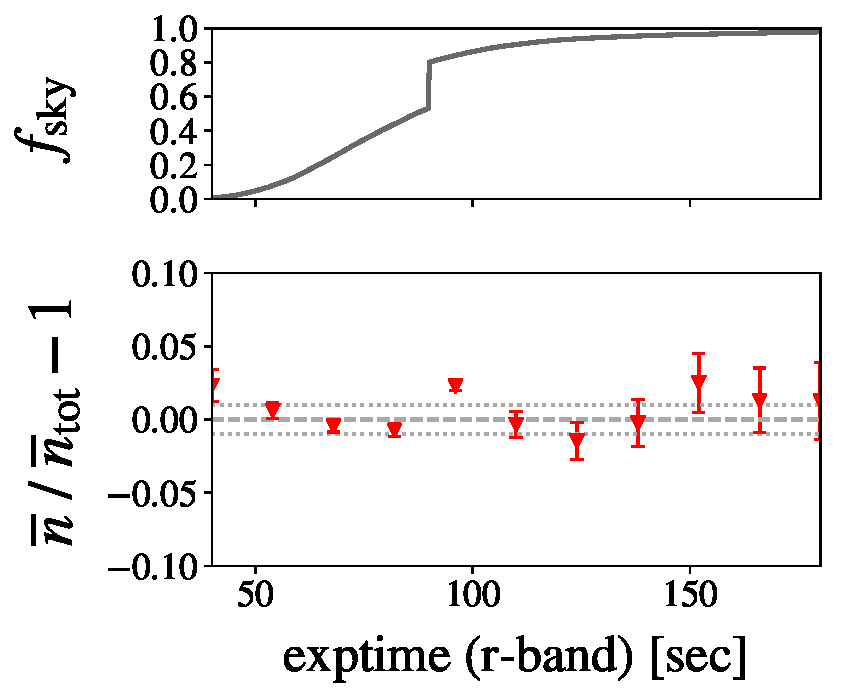
\includegraphics[width=0.24\linewidth]{figures/systematic_trends/exptime_r.pdf}
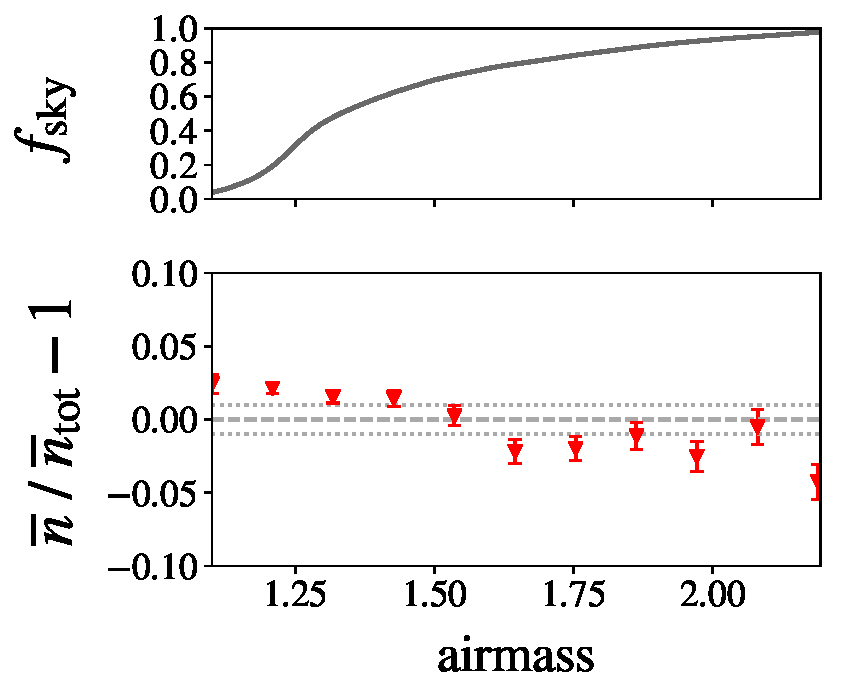
\includegraphics[width=0.24\linewidth]{figures/systematic_trends/airmass.pdf}
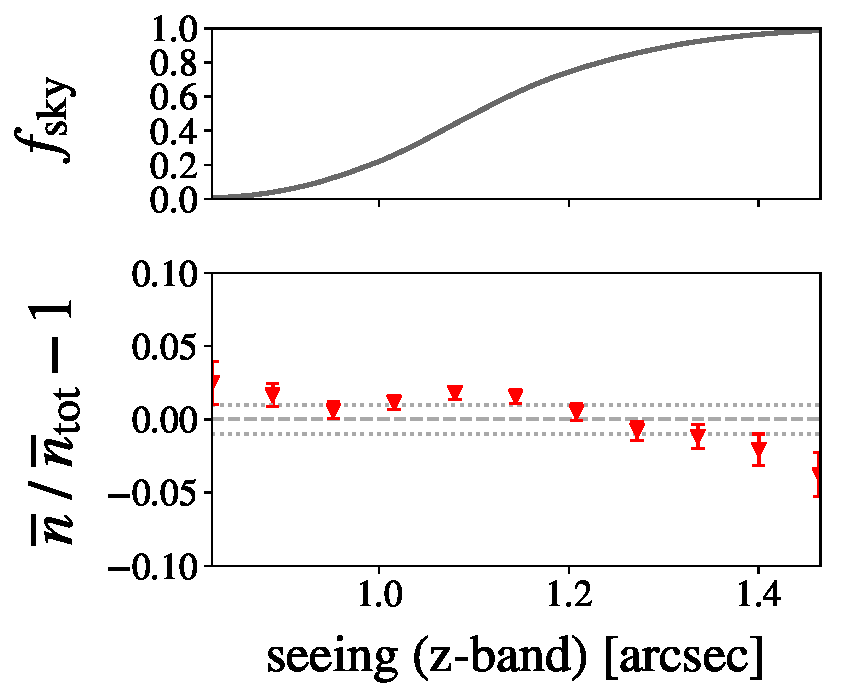
\includegraphics[width=0.24\linewidth]{figures/systematic_trends/seeing_z.pdf}
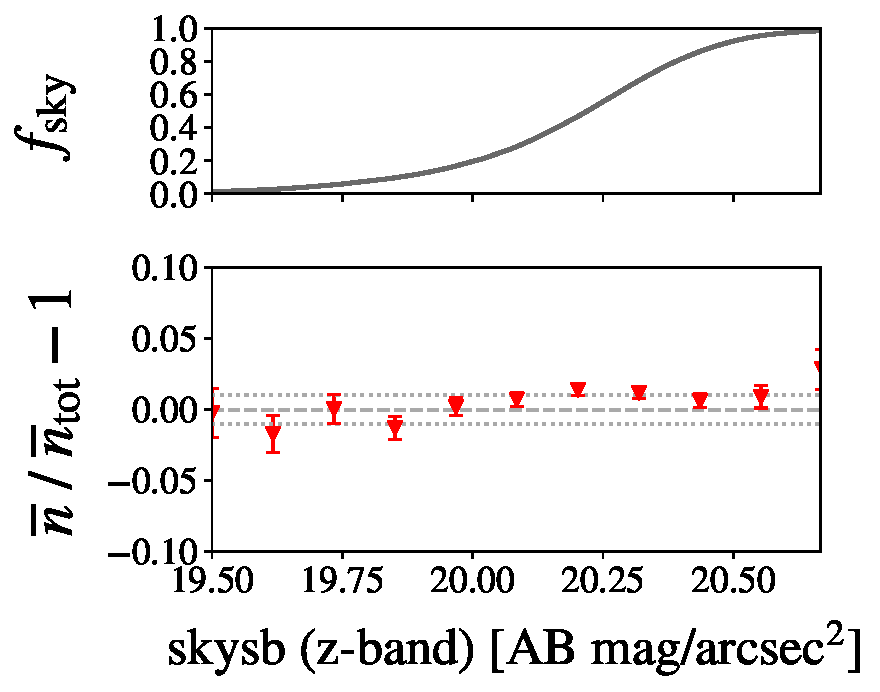
\includegraphics[width=0.24\linewidth]{figures/systematic_trends/skymag_z.pdf}
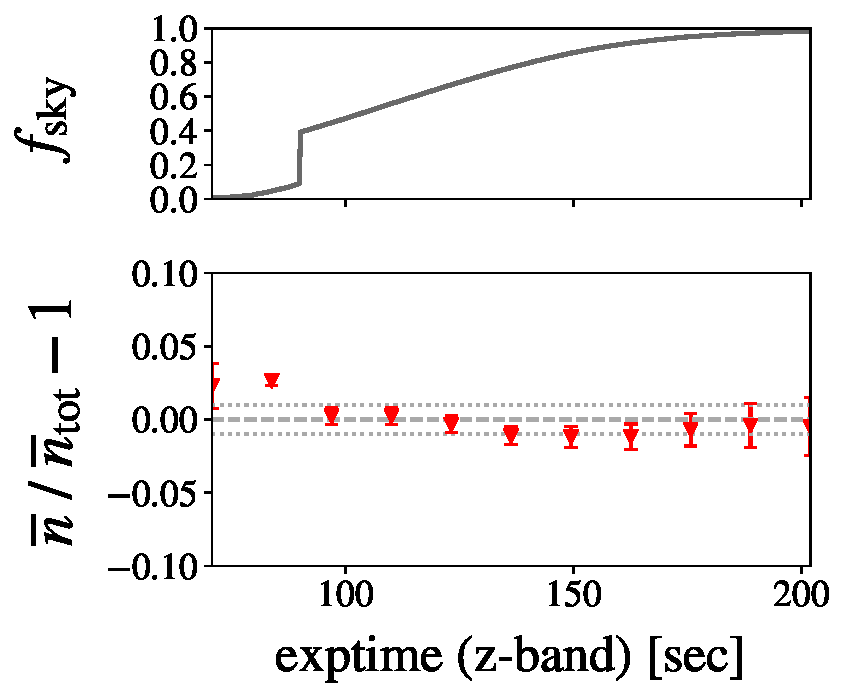
\includegraphics[width=0.24\linewidth]{figures/systematic_trends/exptime_z.pdf}
\caption{Density of LRGs as a function of stellar density, galactic extinction (color excess), airmass, seeing in each optical band, sky subtraction in each optical band, and exposure time in each optical band. Densities and survey properties are smoothed over the scale of the pixelised maps in Figure~\ref{fig:systematic_maps}. The upper panels show the cumulative sky fractions for each survey property, and the dotted lines correspond to $\pm 1\%$ density fluctuations.}
\label{fig:systematic_trends}
\end{figure*}
